\documentclass[conference]{IEEEtran}
\usepackage{amsmath,amssymb,amsfonts}
\usepackage{algorithmic}
\usepackage{algorithm}
\usepackage{array}
\usepackage[caption=false,font=normalsize,labelfont=sf,textfont=sf]{subfig}
\usepackage{textcomp}
\usepackage{stfloats}
\usepackage{url}
\usepackage{verbatim}
\usepackage{graphicx}
\usepackage{xcolor}
\usepackage{cite}

\graphicspath{{figures/}} %set folder for figures


\begin{document}

\title{Anomaly Detection for Time Series Data using VAE-LSTM Model}

\author{
    \IEEEauthorblockN{Randall Fowler}
    \IEEEauthorblockA{\textit{Department of ECE} \\
    \textit{UC Davis}\\
    rlfowler@ucdavis.edu}
    \and
    \IEEEauthorblockN{Conor King}
    \IEEEauthorblockA{\textit{Department of ECE} \\
    \textit{UC Davis}\\
    cfking@ucdavis.edu}
    \and
    \IEEEauthorblockN{Ajay Suresh}
    \IEEEauthorblockA{\textit{Department of ECE} \\
    \textit{UC Davis}\\
    ajsuresh@ucdavis.edu}
}

\maketitle
\thispagestyle{plain}
\pagestyle{plain}

\begin{abstract}
    This paper presents an approach for detecting anomalies in time series data using a hybrid Variational Autoencoder (VAE) and Long Short-Term Memory (LSTM) model. The model leverages the VAE's ability to condense data into a lower-dimensional latent space and the LSTM's capacity for capturing temporal dependencies, enabling precise anomaly detection. Our approach is evaluated on three distinct datasets: Inertial Measurement Unit (IMU) data, synthesized Photoplethysmography (PPG) signals, and Electric Vehicle (EV) drive cycle data. The proposed VAE-LSTM model demonstrates its efficacy in identifying motion artifacts in health monitoring, speed irregularities, and battery voltage anomalies in EVs. Experimental results highlight the model's potential in various applications, though further refinement in thresholding methods and loss functions is suggested to enhance robustness and accuracy.
\end{abstract}

\begin{IEEEkeywords}
Anomaly Detection, VAE, LSTM, Time Series Data, IMU, PPG, EV Drive Cycle, Deep Learning
\end{IEEEkeywords}

\section{Introduction}
Anomalies, often referred to as outliers, are patterns in data that do not conform to a well-defined notion of normal behavior. However, anomalies are not always well-defined, and from the human eye, they may be unnoticeable. In this case, how do you find the problem? This paper dives into a technique for detecting anomalies in time series data by predicting what should happen to the data next. A model is trained to learn the distribution of the data and witness how temporal information may very this distribution.

A VAE is a deep learning model that condenses information into a lower dimensional space than it started as. The idea behind this is that information may be sparse and be difficult to find important features, but this latent space may reduce the sparsity. This latent space can be taken advantage of by making temporal predictions prior to reconstructing the signal. LSTM models contain memory units within their layers to utilize the past and present for future predictions. By predicting on the latent space, data could be more easily interpreted for the defined model before reconstructing the new signal. If the predicted signal is far from what it is, this is a good indication that an anomaly may exist.

Health data is often corrupted by motion artifacts. This is especially true for health data gathered from wearable devices, which are proliferating and an active area of research \cite{conor_ref}. If the health data is to be used to make accurate and useful predictions, it needs to be an accurate representation of the measured variables. Where motion artifacts are present, even if the majority of the data is accurate, the algorithms making use of the data could produce flawed predictions, with potentially serious consequences. Therefore, the ability to systematically identify motion artifacts and other anomalies is of great value. Suspect data can be flagged, or algorithms which focus on reliable data segments can be developed. Areas which would especially benefit from this capability are those involving highly regular time-series data, such as cardiovascular monitoring, sleep disorder analysis, and photo plethysmographs (PPGs), the last of which is one of the main focuses of this paper.

Anomaly detection in EVs can be extremely useful for ensuring the reliability, safety, and efficiency of EVs. Identifying deviations from normal patterns, it helps in early detection of potential issues, preventing costly breakdowns and ensuring optimal performance. While there are a wide variety of applications within the EV space, this report choses to focus on the usage of anomaly detection for vehicle speed and battery voltage as examples.

Anomaly detection for vehicle speed has several potential applications, including:

\begin{itemize}
    \item \textbf{Drivetrain Monitoring:} Detecting anomalies in vehicle speed helps in identifying issues with the drivetrain, including motor performance, transmission, and control systems.
    \item \textbf{Driver Behavior Analysis:} Anomalies in speed patterns can also be used to analyze and improve driver behavior, ensuring safer and more efficient driving practices.
    \item \textbf{Autonomous Driving Systems:} In autonomous vehicles, maintaining consistent speed is crucial. Anomaly detection in speed data helps in ensuring that the autonomous driving system is functioning correctly and safely.
\end{itemize}

Similarly, anomaly detection for battery voltage is also crucial for the following reasons:
\begin{itemize}
    \item \textbf{Battery Health Monitoring:} Detecting anomalies in vehicle speed helps in identifying issues with the drivetrain, including motor performance, transmission, and control systems.
    \item \textbf{Energy Management Systems:} Anomalies in speed patterns can also be used to analyze and improve driver behavior, ensuring safer and more efficient driving practices.
    \item \textbf{Safety and Reliability:} In autonomous vehicles, maintaining consistent speed is crucial. Anomaly detection in speed data helps in ensuring that the autonomous driving system is functioning correctly and safely.
\end{itemize}

\section{Methodology}
Anomaly detection is represented by measuring the reconstruction error from a given deep learning model. For this system, a VAE and LSTM hybrid model is used for finding a latent space with a known distribution and capturing temporal information over time series data. This data is presented in a windowed fashion to locate anomalies within a given window. Evaluation of the anomaly detection will be measured using the harmonic mean of precision and recall (F1 score).

\subsection{Preprocessing}
The nature of the data used for this detection system does not need to be specific, but it does require being time series data. With a given window size, a sliding window will sample the original signal, and the VAE input and output will be equivalent to the size of the window. 

As this data does not need to be labeled, it does need to be clean of noise or anomalies. This is due to the model learning the clean distribution of the data, and after training, the poor reconstruction of a signal will indicate the possibility of an anomaly.


\subsection{Variational Autoencoder}
An autoencoder structure establishes a method for compressing information into a dense latent space. This space is not unique as the original signal can be encoded into a large number of different latent spaces. The VAE addresses this non-regularization issue of the latent space by forcing the space to follow a specific distribution\cite{vae_page}. For most VAEs, this distribution is a normal distribution, and the output of the encoder will be a prediction of mean and standard deviation. Once the distribution of the latent space is known, a sampling will be performed to create a latent vector for the input of the decoder. When the latent space distribution is well formed, the output of the decoder aims to reconstruct the original signal as best as possible.

As the autoencoder represents encoder and decoder models, these structures can be created in a variety of ways. For this project, both will be presented by 1-dimensional convolutional layers with a leaky ReLU activation function and batch normalization. The number of samples per window will decrease while depth increases for every layer in the encoder structure. At the end of the encoder, the samples and depth are flattened and passed to linear layers to condense to the final latent space mean and standard deviation values. Samples from the normal distribution will be given to a decoder that is identical to the encoder, but with transpose convolutional layers to increase the size and decrease the depth. Padding for each layer is forced to maintain a consistent  linear decrease in the number of samples. For this architecture, four convolutional layers are used with a split set of linear layers for the mean and standard deviation prediction.

\subsection{Long Short-Term Memory}
With a sampled latent space created from the encoder, the LSTM takes the current latent vector and attempts to predict the next sample. If the VAE is trained well, it should hold the distribution for the dataset, and the LSTM should learn the temporal differences between each latent window. The LSTM tracks previous outcomes by utilizing memory variables or acting as a state machine. Cell memory and hidden state become the long-term and short-term aspects of the model, and those components carry into the model as inputs \cite{lstm_page}. After each iteration, the memory variables will output to be used by another LSTM layer or dropped before other layers.

A standard LSTM layer contains a tangent activation function, and the PyTorch library does not provide an option to adjust the activation function \cite{lstm_pytorch}. For this reason and the lack of activation function post latent space sampling, a linear layer is placed after the final LSTM layer to adjust for scaling.

\subsection{VAE-LSTM Model Training}
Since the two models hold separate functions for the detection system, the training for the VAE and LSTM are handled separately. Both will use the same training set as the models will be combined after training. Batch size, loss function, and optimizer may vary between the two models.

Loss function can differ greatly as the VAE can be trained with Kullback-Leibler (KL) divergence. This loss relates to the similarity between the latent space distribution and the unit normal distribution \cite{vae_page}. Essentially, it enables the latent space to hold this normal distribution shape. Reconstruction loss is another term that focuses on training the weights regardless of the latent space. The sum of the similarity and reconstruction loss promotes a smooth and continuous latent space while improving signal reconstruction.

The LSTM only needs to focus on the error for prediction on known future samples. This error may be the same as reconstruction loss for the VAE. With the memory components, these need to be initialized properly when training. For each given batch, the batch needs to remain in sequential order, and the memory should be reset if batches are not in order. For predictions on an entire dataset, the memory should only be reset at the very beginning. When resetting, the cell memory and hidden state are initialized with a Normal Xavier Initialization \cite{xavier}. This sets the weights using a normal distribution with a mean of 0 and a variance dependent on the number of inputs and outputs of a layer.

\subsection{Anomaly Detection}
After training, anomalies are detected using the reconstruction error of the predicted sample and thresholding this value. When an anomaly occurs, the model will predict the known distribution and notice the disruption after decoding. The VAE can detect anomalies without the LSTM, but it will be lacking the temporal aspects and recognize the anomaly on reconstruction error alone.

Since the original signal will be windowed prior to input, each window will have an error associated with predicting an anomaly. To represent the anomaly detection in the original signal rather than the windowed version, each data point in the window will be stored in its respective position. Each data point will be the average of all window errors that data point is utilized in. For the first data point in the original signal and first window, this error will be the error of the first window. The second data point will be the average error between the first window and second window. Once the last data point of the first window is reached, this point will be averaged over the same number of windows as the window size, and all following data points will be averaged the same until the final window is reached.

The purpose of averaging error over windows provides a smoother transition between several points where an anomaly would be. It is unlikely that a signal data point will hold an anomaly as typically, an anomaly will occur over a range of time. This issue is also addressed in the next section to increase the score if a section of an anomaly is detected.

\subsection{Evaluation Metrics}
Evaluation of the detection system is handled using an F1 score as this is a measure of precision over sensitivity \cite{f1_page}. Precision is the accuracy of positive predictions, and it is divided by the total positive predictions. Sensitivity, or recall, is the rate of true positives where the number of true positives is divided by the sum of true positives and false negatives. While accuracy of predictions may be a good metric, F1 score considers the distribution of predictions as it is the harmonic mean between the precision and recall.

Since anomalies typically occur in sections of a signal rather than pointwise, assessment per anomaly region could be a better method for measuring true positives. One strategy is to assume any anomaly segment in the ground truth that is detected would be considered a correct detection for that segment, and any point outside of that segment would be treated normally \cite{aug_score}. This method will be referred to as the augmented F1 scoring, and both the regular and augmented F1 score will be evaluated.

\section{Experiments}
Due to the restrained time, the exploration of hyperparameters, architecture, and optimization techniques were limited to first implementations. 

The window size was set to be 100 samples of the original signal with a stride of 1. Each prediction by the LSTM is dedicated to a single window, but since the stride is one, this is a sample-by-sample prediction. Padding for each layer is forced to maintain a consistent linear decrease in the number of samples. Different window sizes should be explored to relate to the different range of time noticed by the model in each moment, but with the difference between signal size and convolutional layers, the exploration was neglected. Four convolutional layers are used in the encoder with a split set of linear layers for the mean and standard deviation prediction, and the decoder layers are identical to the encoder. In the latent space, the LSTM is also given 4 LSTM layers to capture a temporal distribution in the latent space. Number of parameters for the entire detection model was nearly 1.25 million parameters.

For the loss function of both models, mean square error (MSE) is selected for ease. Binary cross entropy (BCE) was considered for loss, but the input and output would be difficult to constrain between 0 and 1. One challenge related to training with similarity loss, KL divergence, as the calculated values did not seem appropriate. This is expected to be a small bug in the implementation, but for the sake of time, it was not used. Without the KL divergence, the VAE would resemble a standard autoencoder.

Training was conducted with varying batch sizes and number of epochs between different datasets, and an Adam optimizer with a learning rate of 4e-4 and betas as 0.9 and 0.95 was selected. 

To explore the robust design of the detection model, three datasets are used for training and testing. IMU dataset consists of motion recordings from multiple sensors to detect movement or changes to the monitoring system. Synthesized PPG data is created from simulating tissue models and aims to detect motion, electromagnetic interference, and other variations of noise. The Electric Vehicle Drive Cycle dataset is synthesized based on referenced data from a Cadillac EV that includes time series data for vehicle speed and battery voltage.

\subsection{Inertial Measurement Unit Dataset}
IMU dataset consists of in-vivo measurements of a device placed on the abdomen of a pregnant woman laying down. The recorded motion comes from 4 sensors with 3 axes each, and all anomalies will consist of movement from the mother, baby, and pressure added to the device. Breathing will be part of the natural signal, but any shift of position could create artifacts. 

Clean data is relatively simple to create as large motion will appear as spikes or y-axis offset, so clean data can be gathered from clipping dirty data, interpolating over the noise, or just making a constant signal with noise. To preserve the in-vivo aspects of the dirty signal, the clean signal is just a clipping of the original, but interpolation would help to preserve length of training. Since training memory is reset per batch, the length of the original signal does not need to be long.

Training with the IMU data follows the same strategy as listed above. The dataset is a combination of multiple channels, but each channel is normalized before training. It’s possible to use each channel to predict anomalies shared between them, but for the sake of time, single channel training is focused on.

\subsection{Synthesized Photoplethysmography Dataset}
Pulse Oximetry is a non-invasive optical technique used to detect blood volume changes in tissue. Light is projected into tissue in one area and light intensity is detected in a different area; as blood is the dominant light absorber in tissue, changes in the intensity correlate with changes in blood volume. Different wavelengths of light are absorbed differently by oxygenated and deoxygenated hemoglobin, and different light source-detector separation distances probe different tissue depths. By using multiple wavelengths and detectors in a single run, the resultant time-series signals are rich in information about blood volume and oxygenation in different areas of the tissue.

The data used in this experiment is synthesized using parameters taken from in-vivo data gathered from pregnant sheep. The time-varying frequency trace and the pulse shapes were taken directly from the sheep-data, while the magnitudes of the different components were determined via Monte Carlo simulation. Thus, the data strongly resembles in-vivo data but is free from anomalies and is suitable for training the VAE-LSTM model. There are four sets of time-series data, each with 10 channels, corresponding to 5 detectors and two wavelengths.

To test the model, the same data is augmented with artificial anomalies. The anomalies are short intervals with a DC shift. The number of anomalies, their positioning, their duration, and their intensity are all determined probabilistically, and are varied slightly between channels, also probabilistically. The data-points affected by the DC shifts are the true anomalies against which the trained VAE-LSTM model is tested. Figure \ref{ck_fig_1} provides an example of the clean data and the anomalous data, with true anomalies highlighted in red.

\begin{figure}[htbp]
    \centering
    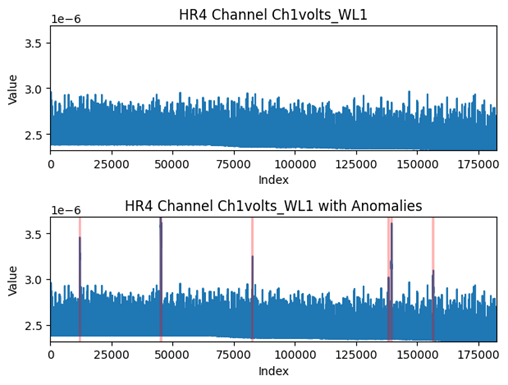
\includegraphics[width=0.5\textwidth]{ck_fig_1.png}
    \caption{Example of synthesized PPG data (top) and the same data with added anomalies (bottom)}
    \label{ck_fig_1}
\end{figure}

\subsection{Electric Vehicle Drive Cycle Dataset}
The dataset consists of time-series data representing the speed of an EV over a drive cycle. The speed data is generated to simulate a realistic driving cycle with a sine wave pattern and added noise to showcase both overall and subtle realistic changes to speed between 0 and 60 mph. The dataset was designed and generated in comparison with actual city and highway drive cycle data from a Cadillac EV. Generating a synthetic dataset here allows for experimentation with further variability of speed and allows for wider coverage while maintaining the frequency of expected changes that a real dataset would see. A visualization of the synthetic speed dataset without anomalies is included in Fig \ref{aj_fig__1}.

\begin{figure}[htbp]
    \centering
    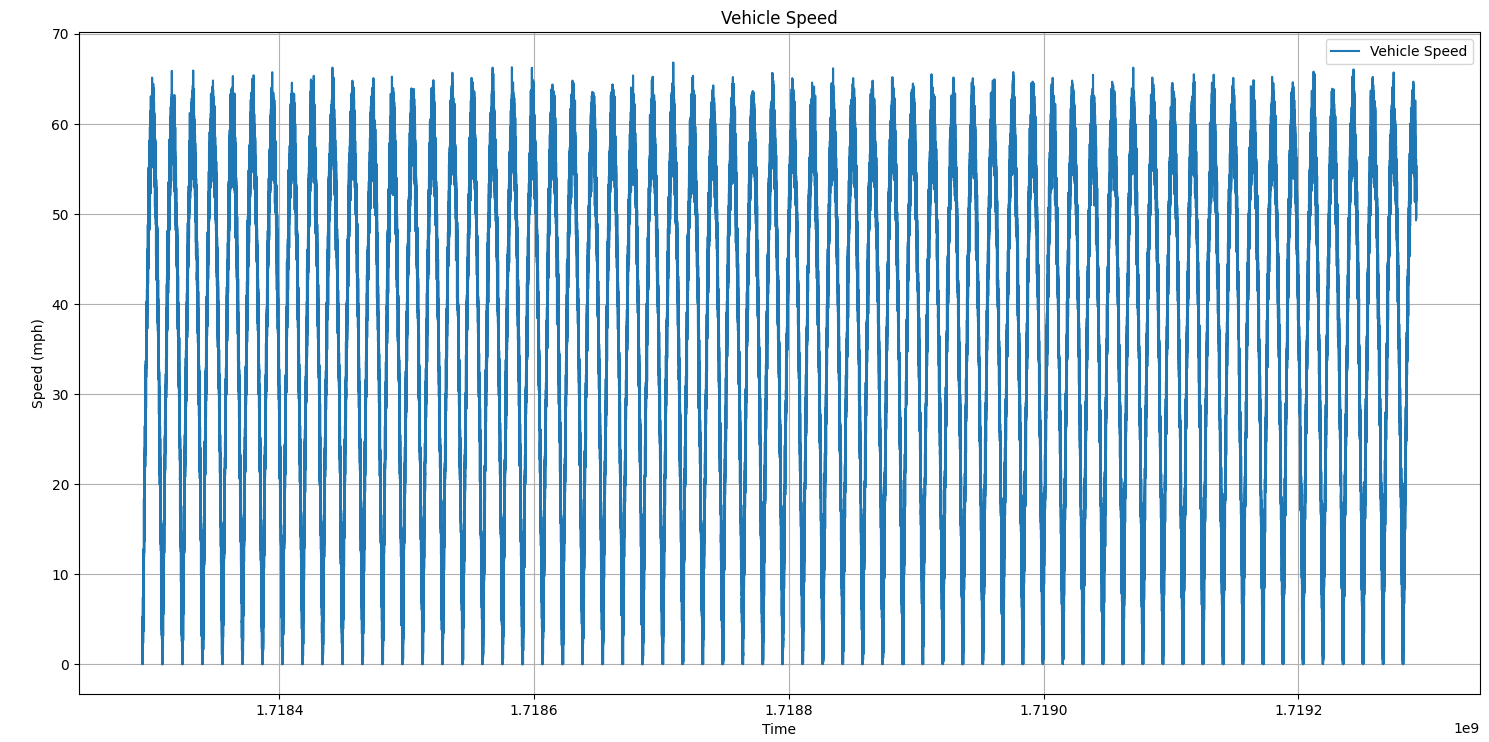
\includegraphics[width=0.5\textwidth]{aj_fig_1.png}
    \caption{Synthetic Data showcasing Vehicle Speed}
    \label{aj_fig__1}
\end{figure}

This dataset represents the voltage levels of an EV battery over a drive cycle. The data is generated to simulate typical voltage patterns for a 400V battery pack, with a sine wave pattern and noise - similarly generated in comparison with actual data obtained from a Cadillac EV. A visualization of the synthetic battery voltage dataset is included in Figure \ref{aj_fig__2}.

\begin{figure}[htbp]
    \centering
    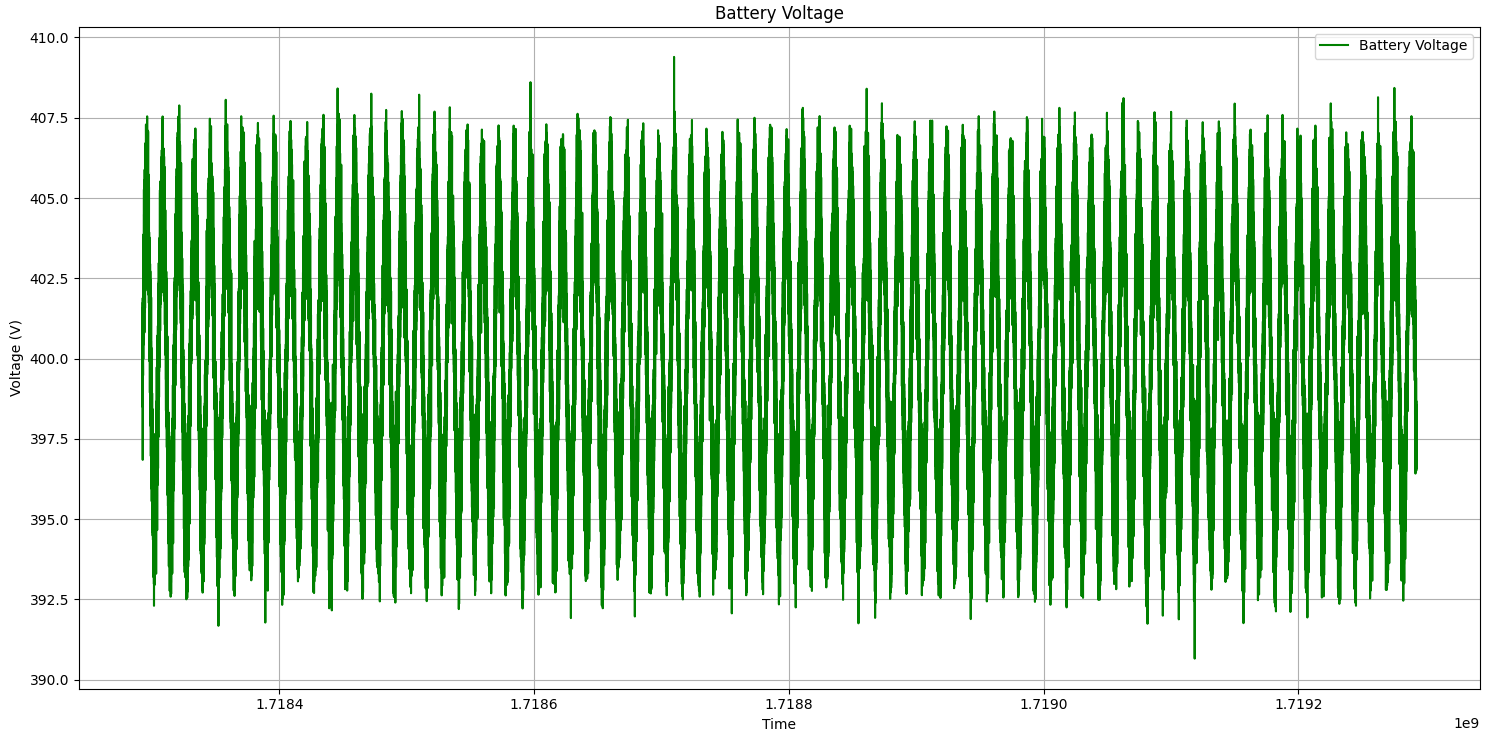
\includegraphics[width=0.5\textwidth]{aj_fig_2.png}
    \caption{Synthetic Data showcasing Battery Pack Voltage}
    \label{aj_fig__2}
\end{figure}

\section{Results}
An issue seen by each of the datasets would relate to the method for thresholding. Methods for determining the error threshold were found by using the mean and standard deviation of each of the signals, but it was determined on each signal separately. This meant that for a signal with little to no anomalies, the error threshold would be very small and over detect the number of anomalies.

In most results, the augmented F1 score used for determined the error threshold proved to be better than the normal F1 score. This may be flawed due to the issues in training and occasional large number of anomalies detected, but it did prove to be useful. 

\subsection{Inertial Measurement Unit}
For the IMU, a more extensive search was performed to find any changes amongst batch size, number of epochs, and size of the latent space. It appeared that changing the size of the latent space did not improve the predictions, but this should be investigated again with improvements to the loss functions. All examples provided will have a latent space of 6 if not specified. Note that the anomalies were labeled manually by what was thought to be issues in the data. This could vary the F1 scoring, but detected anomalies could also be visually compared in this paper.

Figure \ref{rf_fig_1} provides the F1 scoring gathered from the evaluation, and a large threshold appears to have better results. This should be expected as Figure \ref{rf_fig_2} shows a few large anomalies present, and with larger anomalies, the threshold should be large to separate the normal signal error to the large changes. The ground truth anomalies may be mismarked as the detected anomalies do appear to have good results. These results come from a model trained with 20 epochs and a batch size of 32, and the best augmented F1 score is used to find the threshold.

\begin{figure}[htbp]
    \centering
    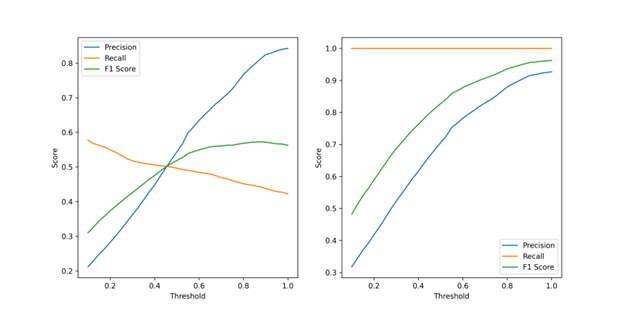
\includegraphics[width=0.5\textwidth]{rf_fig_1.png}
    \caption{}
    \label{rf_fig_1}
\end{figure}

\begin{figure}[htbp]
    \centering
    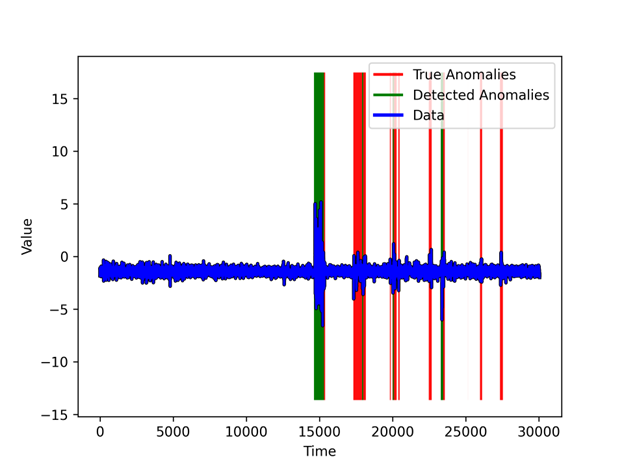
\includegraphics[width=0.5\textwidth]{rf_fig_2.png}
    \caption{}
    \label{rf_fig_2}
\end{figure}

For the next example, the same test file was used with the same parameters except the latent space was increased to 12. Figures \ref{rf_fig_3} and \ref{rf_fig_4} show the F1 score and anomaly plot respectively. The F1 score does look vastly smaller than the one in Figure \ref{rf_fig_1}, and this would be due to the poor precision of the model. It is thought that the model did not train well, and most windows had a less deterministic error distribution. 

\begin{figure}[htbp]
    \centering
    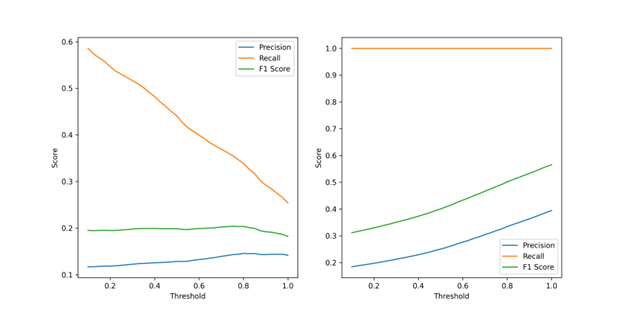
\includegraphics[width=0.5\textwidth]{rf_fig_3.png}
    \caption{}
    \label{rf_fig_3}
\end{figure}

\begin{figure}[htbp]
    \centering
    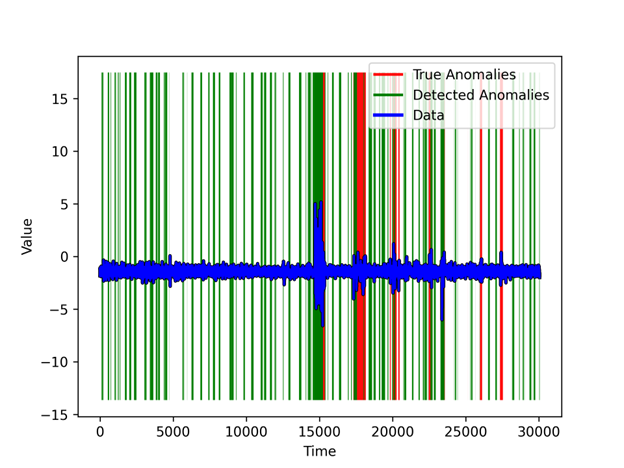
\includegraphics[width=0.5\textwidth]{rf_fig_4.png}
    \caption{}
    \label{rf_fig_4}
\end{figure}

The last example retains the batch size of 32 and latent space of 6, but 100 epochs were used for training the model. Figures \ref{rf_fig_5} to \ref{rf_fig_7} display the results of this model as the scoring has a slightly similar shape, but Figures \ref{rf_fig_6} and \ref{rf_fig_7} compare the normal scoring to augmented. Normal scoring does not perform well as a lower threshold has the larger score. Intuitively, the larger threshold should usually provide better anomaly detection unless there are many anomalies present. Augmented scoring does have similar results to \ref{rf_fig_2}, but still does not perform as well.

\begin{figure}[htbp]
    \centering
    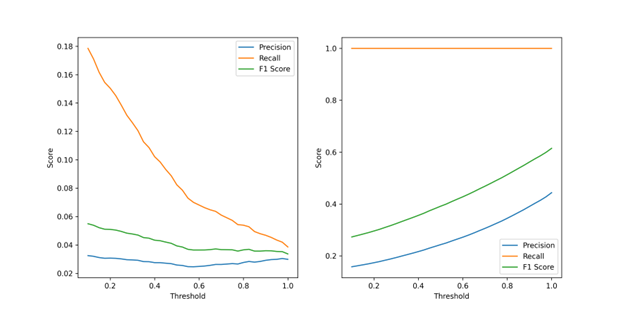
\includegraphics[width=0.5\textwidth]{rf_fig_5.png}
    \caption{}
    \label{rf_fig_5}
\end{figure}

\begin{figure}[htbp]
    \centering
    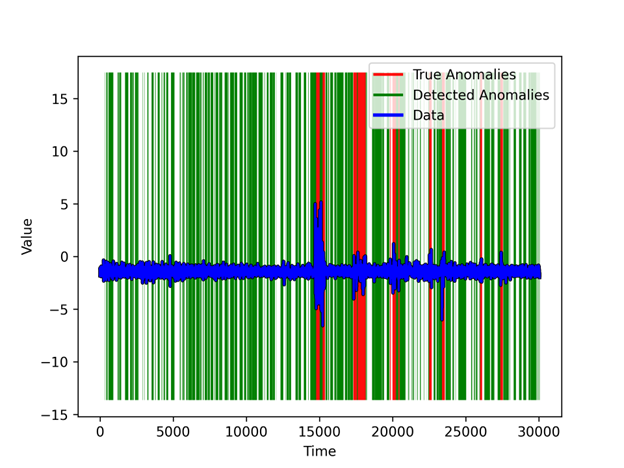
\includegraphics[width=0.5\textwidth]{rf_fig_6.png}
    \caption{}
    \label{rf_fig_6}
\end{figure}

\begin{figure}[htbp]
    \centering
    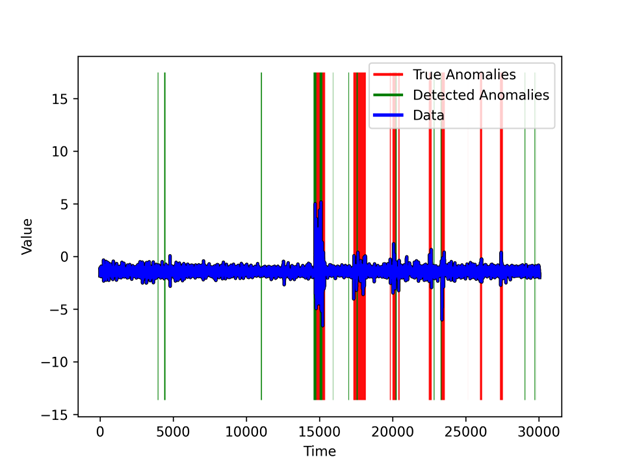
\includegraphics[width=0.5\textwidth]{rf_fig_7.png}
    \caption{}
    \label{rf_fig_7}
\end{figure}


\subsection{Synthesized Photoplethysmography}
The performance of the VAE-LSTM model on the synthesized PPG data with artificial anomalies was somewhat varied. As expected, it depends enormously on the chosen threshold value.

When the best threshold without anomaly augmentation is used, the performance is generally good, as exhibited by Figure \ref{ck_fig_2}. The small anomaly to the far right of the data is not detected, but its magnitude is so small that that seems reasonable.

\begin{figure}[htbp]
    \centering
    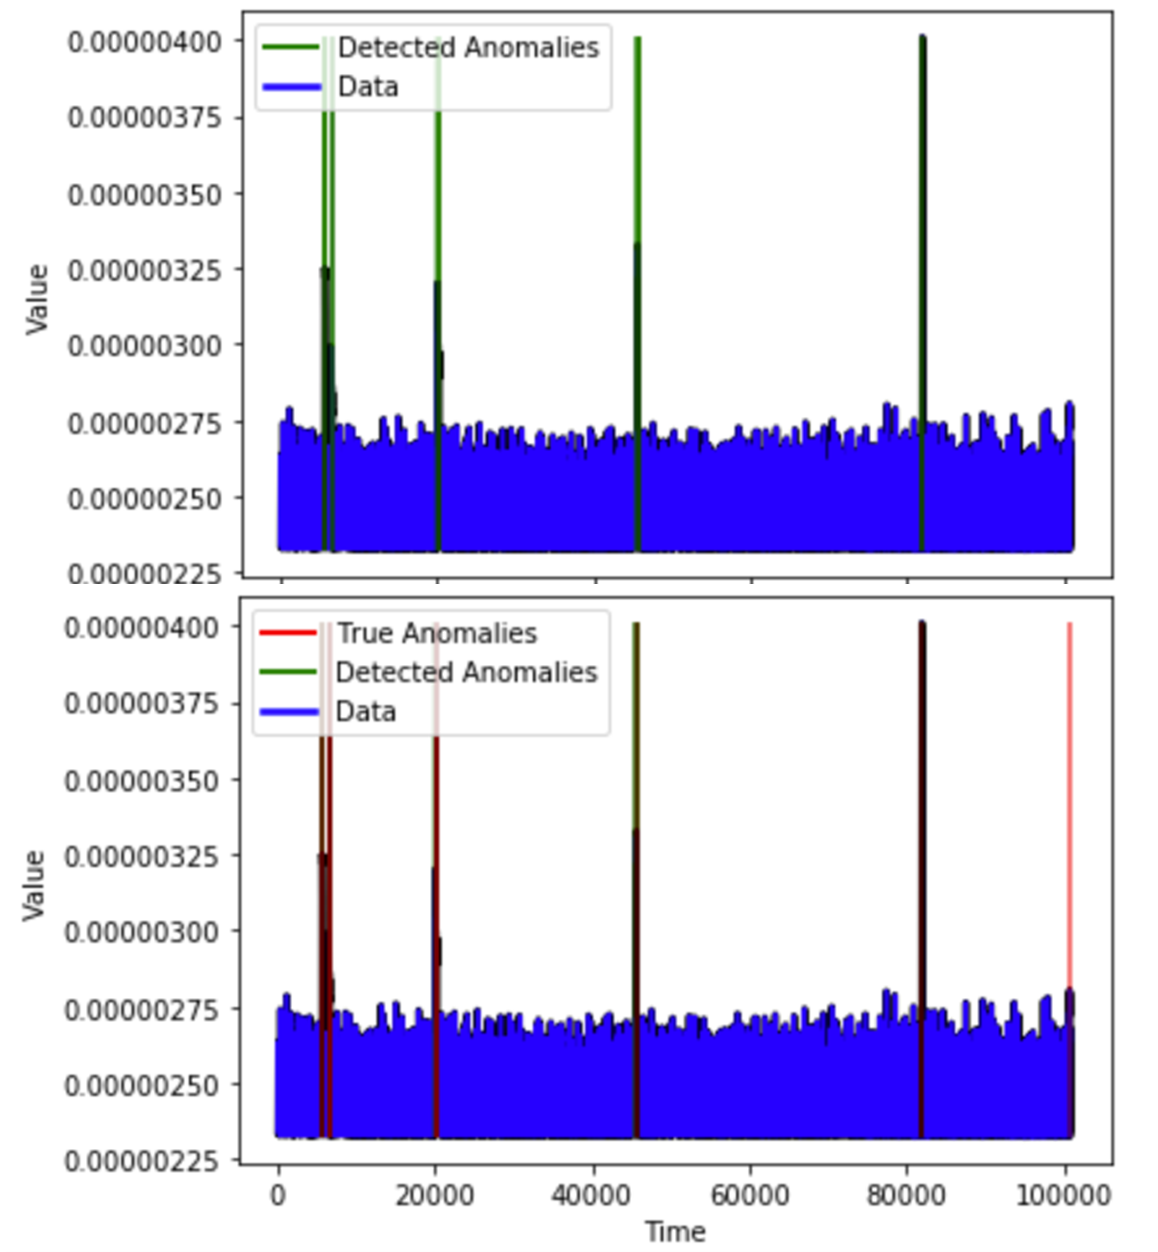
\includegraphics[width=0.5\textwidth]{ck_fig_2.png}
    \caption{Example of good performance of the model. Slight false negative on the far right}
    \label{ck_fig_2}
\end{figure}

However, sometimes that thresholding level causes the model to suffer from extreme overprediction, and the best threshold found during testing with anomaly augmentation works better, as in Figure \ref{ck_fig_3}.

\begin{figure}[htbp]
    \centering
    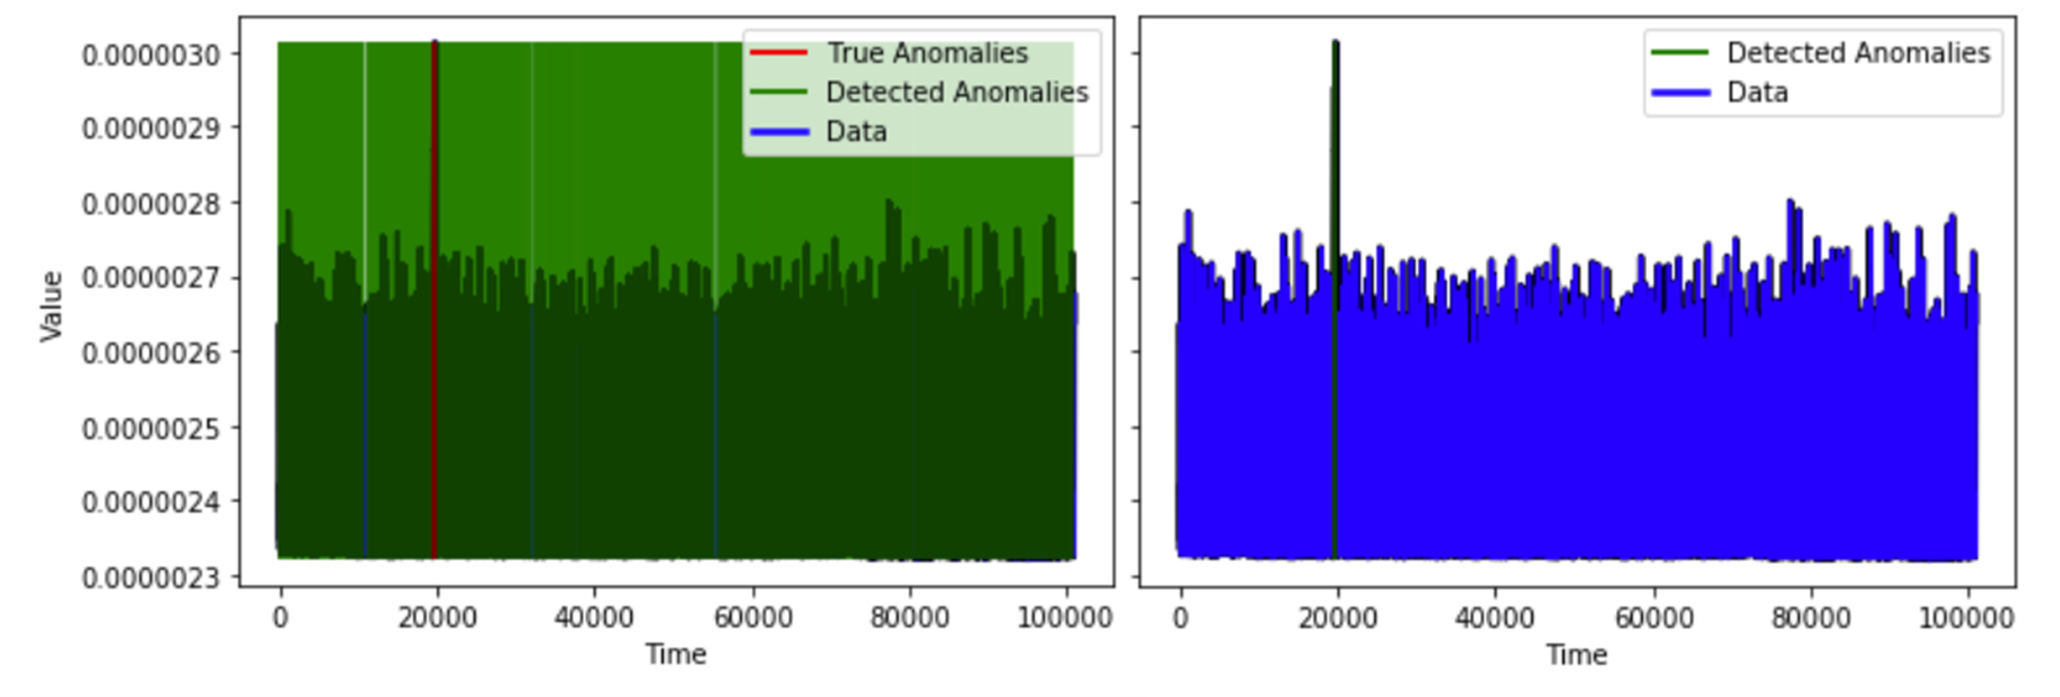
\includegraphics[width=0.5\textwidth]{ck_fig_3.png}
    \caption{Left: Best threshold w/o augmentation. Right: Best threshold w/ augmentation}
    \label{ck_fig_3}
\end{figure}

Often, a value between the two “best” values actually produced the best results. In the case of Figure \ref{ck_fig_4}, the best threshold when augmentation was not used as 0.1 (top), and the best threshold when augmentation was used was 5.5 (bottom). The top plot shows extreme overprediction of anomalies while the bottom misses the leftmost anomaly and a smaller anomaly in the middle. The middle plot, using a hand-selected threshold of 0.5, successfully finds the anomalies without overpredicting.

Overall, these results suggest that the model learned the structure of the synthesized PPG data well and is able to reliably predict anomalies when a suitable threshold is chosen. However, finding a systematic way of selecting a good threshold proves more challenging.

\begin{figure}[htbp]
    \centering
    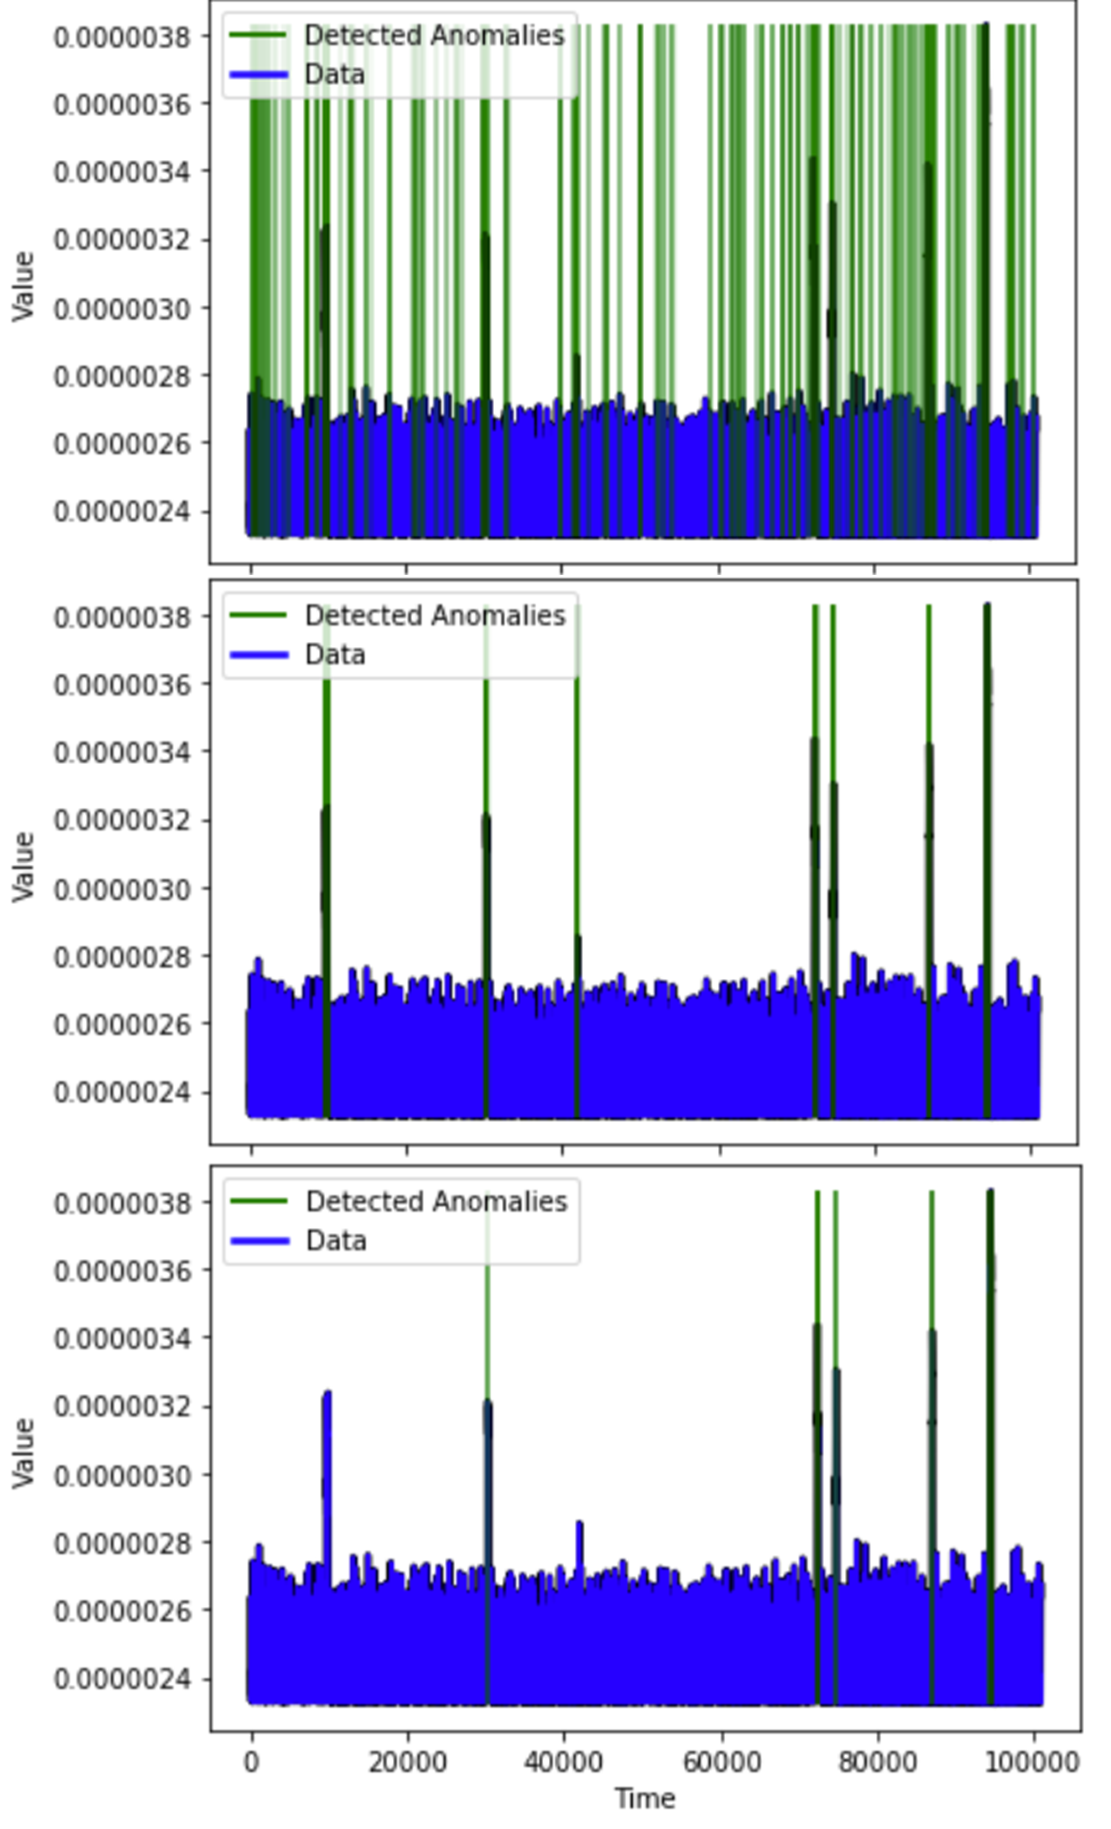
\includegraphics[width=0.5\textwidth]{ck_fig_4.png}
    \caption{A threshold value between the two ostensible best values produces better results than either}
    \label{ck_fig_4}
\end{figure}

\subsection{Electric Vehicle Drive Cycle}
\subsubsection{Vehicle Speed}
Figure \ref{aj_fig__3} shows the synthesized and normalized test dataset to evaluate the VAE + LSTM model to detect anomalies within vehicle speed. Random data points were selected and a speed spike of 20 to 40 mph were introduced to simulate an actual spike in vehicle speed that wouldn’t normally occur during a regular drive cycle. The goal was to fine tune the model to be able to detect just the 5 red dots (speed spikes) that are visible in the figure.

\begin{figure}[htbp]
    \centering
    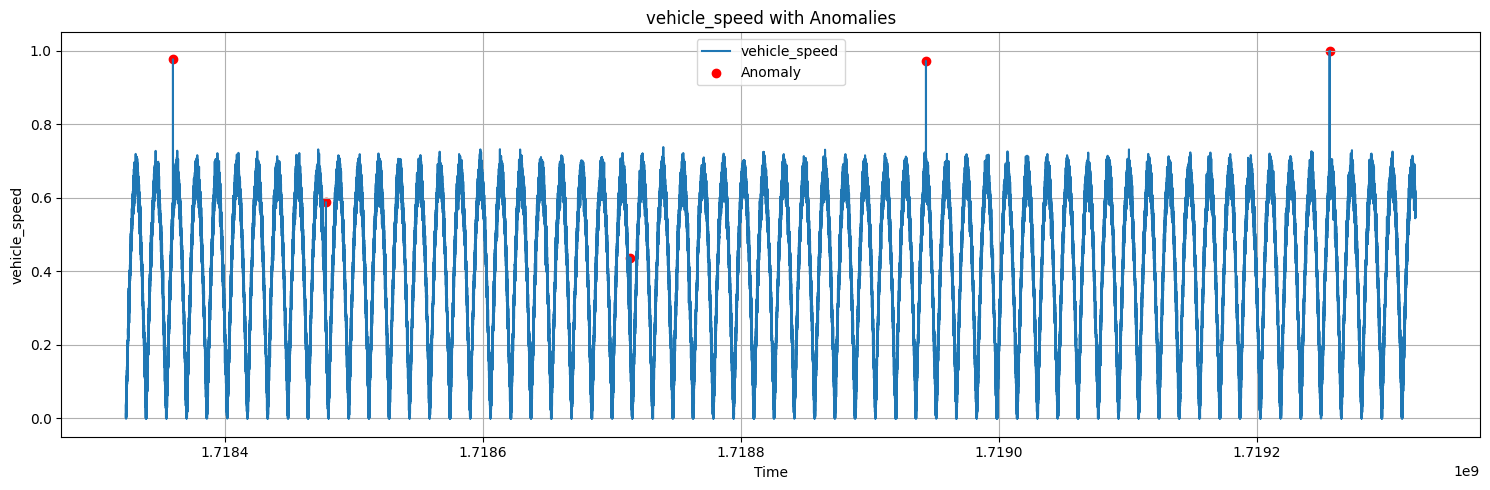
\includegraphics[width=0.5\textwidth]{aj_fig_3.png}
    \caption{Vehicle Speed with introduced anomalies (spikes in speed)}
    \label{aj_fig__3}
\end{figure}

The results of Figure (\ref{aj_fig__4}) showcase an overdetection of anomalies within the dataset as showcased by the green lines in the figure. Although this has been a common issue amongst all tested datasets, in this case, the variations in speed demonstrate realistic changes that are fairly noisy - which can be difficult to separate from a real anomaly unless further tuning is performed. 

\begin{figure}[htbp]
    \centering
    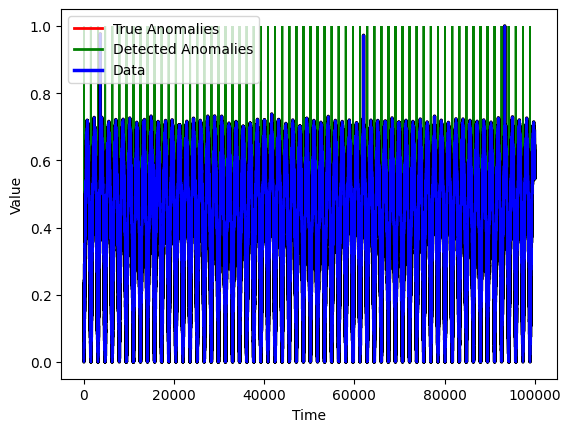
\includegraphics[width=0.5\textwidth]{aj_fig_4.png}
    \caption{Results of VAE + LSTM Anomaly Detection for Vehicle speed}
    \label{aj_fig__4}
\end{figure}

\subsubsection{Battery Voltage}
Figure \ref{aj_fig__5} shows the synthesized and normalized test dataset to evaluate the VAE + LSTM model to detect anomalies for battery pack voltage. In the context of this experiment, anomalies in battery voltage are simulated by introducing sudden drops in the voltage levels. The drop in voltage is simulated by subtracting a random value (e.g., between 5V to 10V) from the current voltage at the selected anomaly points - which are above the realistic thresholds of a voltage drop during regular operation.

\begin{figure}[htbp]
    \centering
    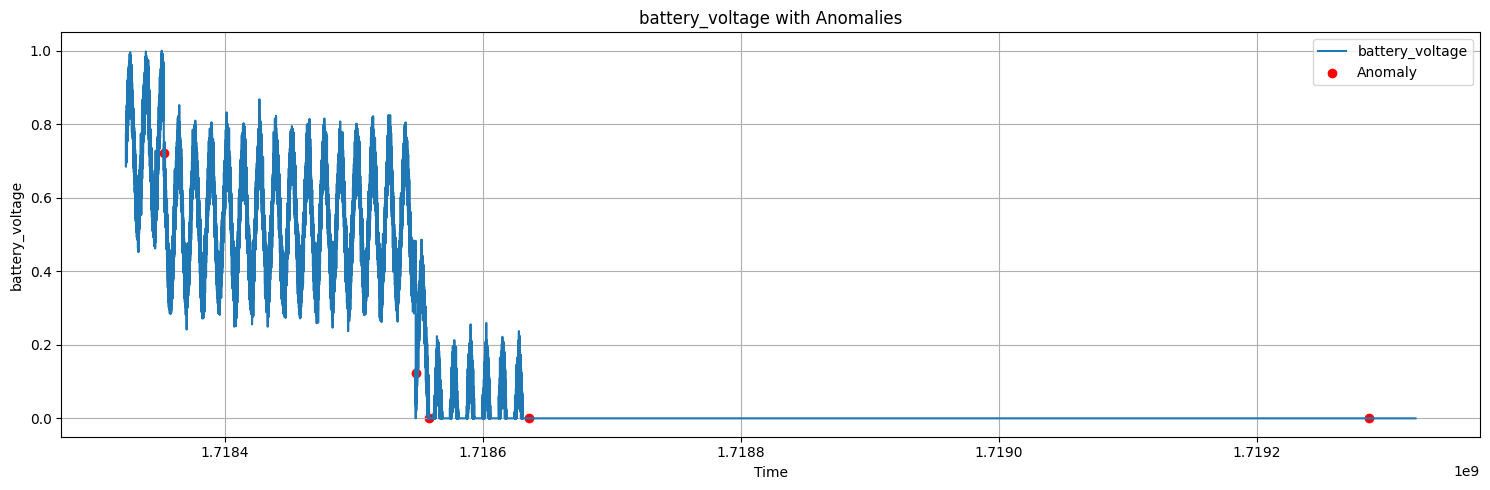
\includegraphics[width=0.5\textwidth]{aj_fig_5.png}
    \caption{Battery Pack Voltage with introduced anomalies (sudden drops in voltage)}
    \label{aj_fig__5}
\end{figure}

\begin{figure}[htbp]
    \centering
    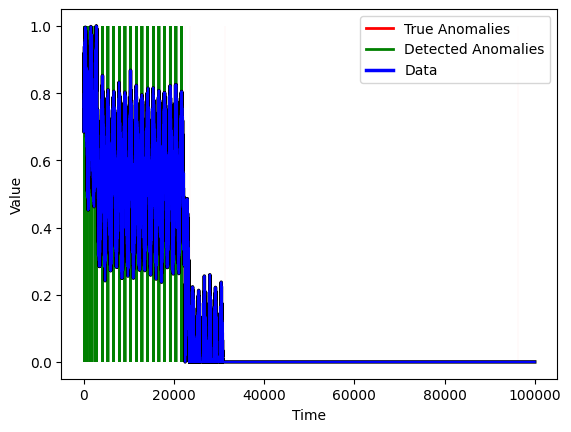
\includegraphics[width=0.5\textwidth]{aj_fig_6.png}
    \caption{Results of VAE + LSTM Anomaly Detection for Battery Pack Voltage}
    \label{aj_fig__6}
\end{figure}

As with the previous results, this dataset also showcases an overdetection of anomalies with some anomalies on the lower range going undetected (lack of green lines after time = 20,000, where at least 2 are expected). 

\section{Conclusion}
The architecture provided shows promise for performing well when detecting anomalies. It appears that the model training lacks stability due to the VAE loss function. Occasionally, the model trains well and the error distribution appears to be good. In the event the model performs well, thresholding is another issue to be addressed. Instead of optimizing the threshold for every signal, thresholding should be determined with a test set to find the minimum error that an anomaly occurs at. These results are not satisfactory, but a path is clear to achieve desirable performance.

\subsection{Future Work}
Many of the issues in this project have been noted throughout the paper, and for future work, these issues would need to be addressed. Loss function should be further explored and resolve the KL divergence term of the VAE loss. BCE could replace the reconstruction error for both models, but both sides of the model would need to be scaled between 0 and 1. The problem with this scaling would be in the final output of the system as the original signal needs to be scaled properly for every signal.

Evaluation could be improved to compare accuracy, F1 score, and display the error distribution for each sample in the signal. This could provide more intuition as F1 score is not an insightful metric, but it could still be useful for optimizing the threshold. The threshold would also need to be searched over many test signals and left as a constant. Currently, the threshold varies per signal, and this is not a good method with a varying number of anomalies. These anomalies should be better labeled, and this can be done by noting the region and interpolating if starting with dirty data. Some datasets will be difficult to remove or add artifacts, but this could be a project by itself.

One mistake recently found would relate to the data used in the LSTM as it currently does not predict new windows. The mistake was that it tries to learn the mold of the latent space and scale errors larger if they are noticed to be out of the distribution. This may be a good strategy, but it contradicts temporal information by outputting the same input at the same time. A set of linear layers could do this, so an improvement would be to fix the output data comparison to be the next window rather than current.

This system is fully capable of handling multichannel inputs, so predicting anomalies over multiple channels could be useful. It has not been explored and their may be bugs in the current implementation.


\section*{Acknowledgment}
The authors would like to thank Dr. Yubei Chen for his guidance and support on this course project.

\section*{Contributions}
Randall Fowler developed the models, evaluation methods, and experimented with the IMU dataset. 
Conor King experimented with the synthesized PPG dataset. 
Ajay Suresh experimented with the EV drive cycle dataset. 
All authors contributed to the writing of the paper.

\begin{thebibliography}{1}
\bibliographystyle{IEEEtran}

\bibitem{ref1}
Citation 1

\bibitem{ref2}
Citation 2

\bibitem{ref3}
Citation 3

\bibitem{ref4}
Citation 4

\bibitem{ref5}
Citation 5

\end{thebibliography}

\end{document}